%% ID: on_ice
%% TITLE: On Ice
%% TYPE: question
%% QUESTIONTYPE: numeric
%% CONCEPTS: newtonii, eq_of_motion_diff, vectors, resolving_vectors
%% VIDEOS: O1979PIIQ3a_Part_a.mov, O1979PIIQ3a_part_b.mov
%% LEVEL: 2
%% TOPIC: mechanics/dynamics
%% ORDER: 5

\begin{problem}[O1979PIIQ3a]
{A rock is resting on a horizontal sheet of ice and acted on by two forces of magnitudes \quantity{15}{N} and \quantity{20}{N}, in perpendicular directions North and East respectively. The friction between the rock and the ice is negligible.
\begin{enumerate}
	\item The rock accelerates at \quantity{4.0}{m\,s$\sup{-2}$}; find the direction in which it moves with respect to North. What is the mass of the rock? \answer{Direction}{53.13}  \answer{m}{6.25}
	\item The forces continue to act so that the rock moves in a straight line for \quantity{6.0}{s}. Calculate the velocity acquired by the rock in this time, and also the distance it has travelled. \answer{v}{24.00}  \answer{s}{72.00}
\end{enumerate}
Write your answer to two decimal places.}
{\stress{Adapted with permission from UCLES, O Level Physics, June 1979, Paper 2, Question 3.}}
{\begin{enumerate}
	\item The components of the forces can be drawn on a diagram with North and East at a perpendicular, as in Figure \ref{fig:Dynamics_vtr_forces}, followed by simple trigonometry to find the direction of the resultant. 
\begin{figure}[h]
	\centering
	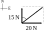
\includegraphics[width=0.2\textwidth]{../../../figures/Dynamics_vtr_forces.eps}
	\caption{}
	\label{fig:Dynamics_vtr_forces}
\end{figure}

The resultant force, denoted by the double headed arrow, is at an angle to the direction of North which can be found by using trigonometry within the top right angled triangle:
	\begin{equation*}\tan(\theta)=\frac{20}{15} = \frac{4}{3} \end{equation*}
	\begin{equation*}\theta = \arctan\left(\frac{4}{3}\right) = 53.1^{\circ} \:\textrm{ from North.}\end{equation*}

To find the mass, use Newton's Second Law: $\vtr{F} = m\vtr{a}$, with the magnitude of the resultant force $F = \sqrt{15^{2} + 20^{2}} \textrm{ N} = 25 \textrm{ N}$, giving: 
\begin{equation*}m = \frac{F}{a} = \frac{25}{4} = 6.25 \textrm{ kg} \end{equation*}
	\item There is a constant acceleration, so the equation $v = u + at$ can be used to find velocity: 
	\begin{equation*} v = [0 + (4)(6)] \textrm{ ms}^{-1} = 24 \textrm{ ms}^{-1} \end{equation*}

As the rock has a constant acceleration, the distance travelled is the average velocity times time. This is also the area under the graph on a velocity/time plot:
	\begin{equation*}\frac{1}{2}(24)(6) = 72 \textrm{ m} \end{equation*}
Alternatively, SUVAT can be employed again:
	\begin{equation*}s = ut + \frac{1}{2}at^{2} = (0)(6) + \frac{1}{2}(4)(6^{2}) = 72 \textrm{ m} \end{equation*}

\end{enumerate}
}
\end{problem}